\chapter{Testy i ocena wyników}
\label{cha:testy_i_ocena_wynikow}
%TODO A nie robił Pan w innnych też ?(dodane RGB)

%TODO--- Tutaj planuję opis poniższych zdjęć (szczególnie histogramów) wraz z wnioskami, że możliwa jest skuteczna detekcja czerwonego znacznika na podstawie składowej Cr.
%TODO OK. Choć trzeba się wytłumaczyć z czerwonego...(wykonane)

%TODO Wnioski no i coś o tym progu - choć pewnie stały.(wykonane)
\section{Wybór znacznika} 
\label{sec:wybor_znacznika}
Autonomiczne lądowanie drona w~oparciu o~system wizyjny wymaga wyposażenia lądowiska w~marker. Jego wygląd musi umożliwiać łatwą detekcję miejsca lądowania. Z~powodu wykonywania operacji na~zewnątrz, znacznik powinien również ułatwiać znalezienie go~w~zmiennych warunkach (zachmurzenie, cień).
\subsection{Kształt}
\label{subsec:ksztalt} 
Detekcja kształtów może być realizowana na~różne sposoby. Najprostszym jest progowanie współczynników kształtu, do~bardziej zaawansowanych należy wyspecjalizowana deskrypcja cech (SIFT, SURF, HOG) i~użycie klasyfikatorów (kNN, SVM, sieci neuronowe). W~implementowanej pierwszej wersji systemu zdecydowano się na~klasyfikację przy użyciu współczynnika kształtu.\\
Cechami obiektu łatwymi do~wyliczenia w~systemie potokowym są~pole figury i~najmniejszy prostokąt, w~którym figura się mieści. Postanowiono zatem wykorzystać współczynnik kształtu przedstawiony we~wzorze \ref{eq:wspolczynnik}.\\
\begin{equation} \label{eq:wspolczynnik}
W=\frac{P_p}{P_o}
\end{equation}
Gdzie:
\begin{eqwhere}[2cm]
	\item[$W$] współczynnik kształtu,
	\item[$P_p$] pole prostokąta otaczającego,
	\item[$P_o$] pole obiektu.
\end{eqwhere}
Aby~taki współczynnik umożliwiał detekcję należało dobrać odpowiedni kształt znacznika. Zdecydowano się na~krzyż, gdyż przy każdej jego orientacji pole prostokąta jest znacznie większe od~pola obiektu.
\subsection{Kolor}
\label{subsec:kolor}
Kolor znacznika powinien umożliwiać łatwe wykrycie jego kształtu. Z~tego powodu pożądane jest silne skontrastowanie figury i~tła. Najbardziej naturalnym rozwiązaniem jest rozważenie kontrastu w~przestrzeni barw RGB, gdyż taki sygnał jest dostarczany przez kamerę.\\
\begin{figure}[h]
	\centering
	\begin{subfigure}{0.4\textwidth}
		\centering
		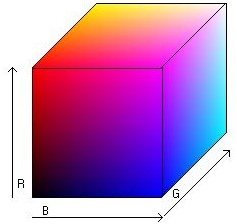
\includegraphics[width=0.5\textwidth]{szescian_rgb.jpg}
		\caption{Przedstawienie przestrzeni barw RGB w~postaci sześcianu \cite{obrazek_rgb}}
		\label{fig:szescian_rgb}
	\end{subfigure}%
	\begin{subfigure}{0.4\textwidth}
		\centering
		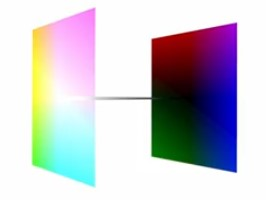
\includegraphics[width=0.5\textwidth]{szescian_ycbcr.jpg}
		\caption{Przekroje sześcianu przestrzeni YCbCr \cite{obrazek_ycbcr}}
		\label{fig:szescian_ycbcr}
	\end{subfigure}%
	\caption{Modele przestrzeni RGB i YCbCr}
	\label{fig:modele_przestrzeni}
\end{figure}
W~przestrzeni RGB każdy piksel opisywany jest przez trzy składowe: czerwoną, zieloną i~niebieską. Możliwe jest przedstawienie tego systemu w~formie sześcianu (Rys. \ref{fig:szescian_rgb}). Można wyznaczyć przekątną łączącą punkty, dla których wszystkie współrzędne są~identyczne. Rozciąga się ona od~czarnego w~początku układu współrzędnych, do~białego dla~maksymalnych wartości składowych, przechodząc przez różne stopnie szarości. Wykorzystanie dużej odległości między kolorami i~użycie czarno-białego znacznika wydaje się najprostszym pomysłem.\\
 Do testów przygotowano czarny znacznik na~białym tle. Kamerą PCAM 5C wykonano trzy zdjęcia przy różnym poziomie oświetlenia (Rys. \ref{fig:osw1}, \ref{fig:osw2}, \ref{fig:osw3}). Po~przejściu na~obraz w~skali szarości, posługując się narzędziem roipoly w~programie Matlab, obliczono histogramy obszaru znacznika (Rys. \ref{fig:bw_hist1}, \ref{fig:bw_hist2}, \ref{fig:bw_hist3}).\\
 \begin{figure}
 	\centering
 	\begin{subfigure}{0.4\textwidth}
 		\centering
 		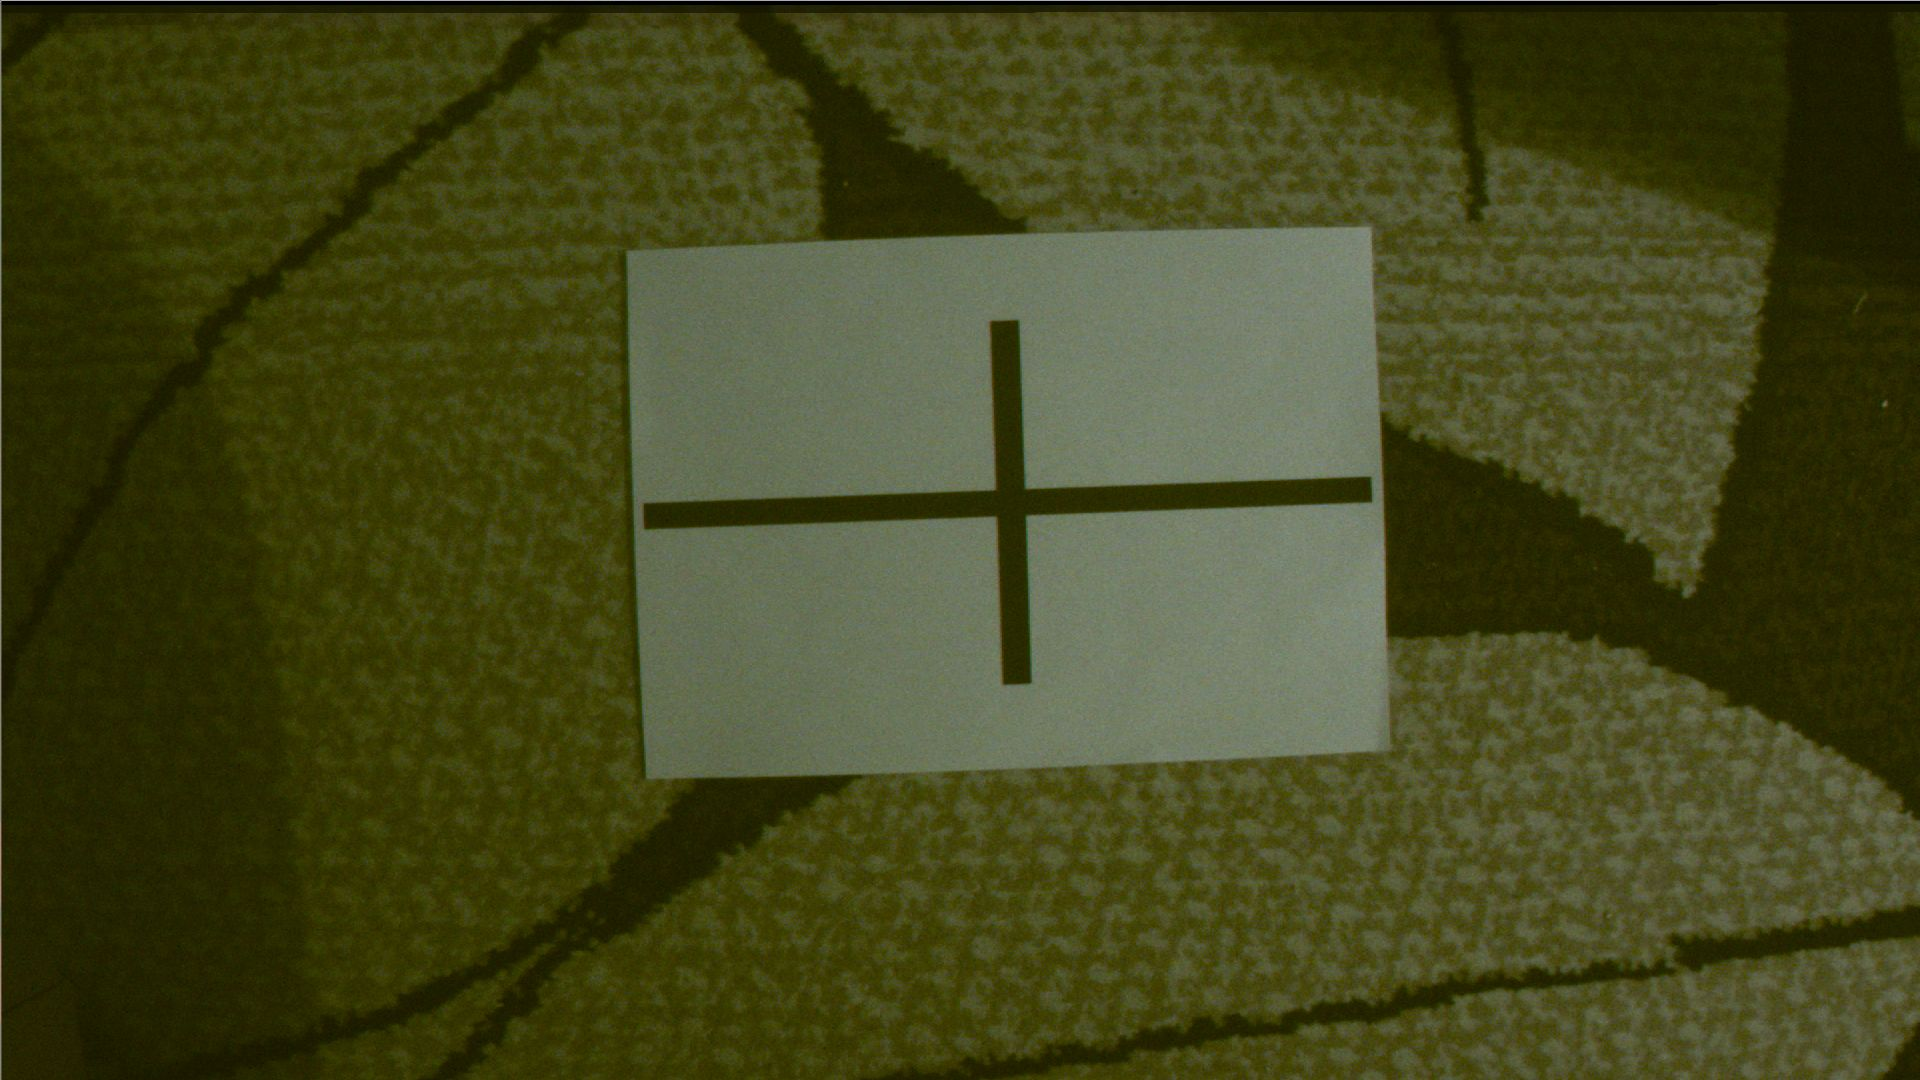
\includegraphics[width=0.98\textwidth]{rgb_ciemny.jpg}
 		\caption{}
 		\label{fig:osw1}
 	\end{subfigure}%
 	\begin{subfigure}{0.55\textwidth}
 		\centering
 		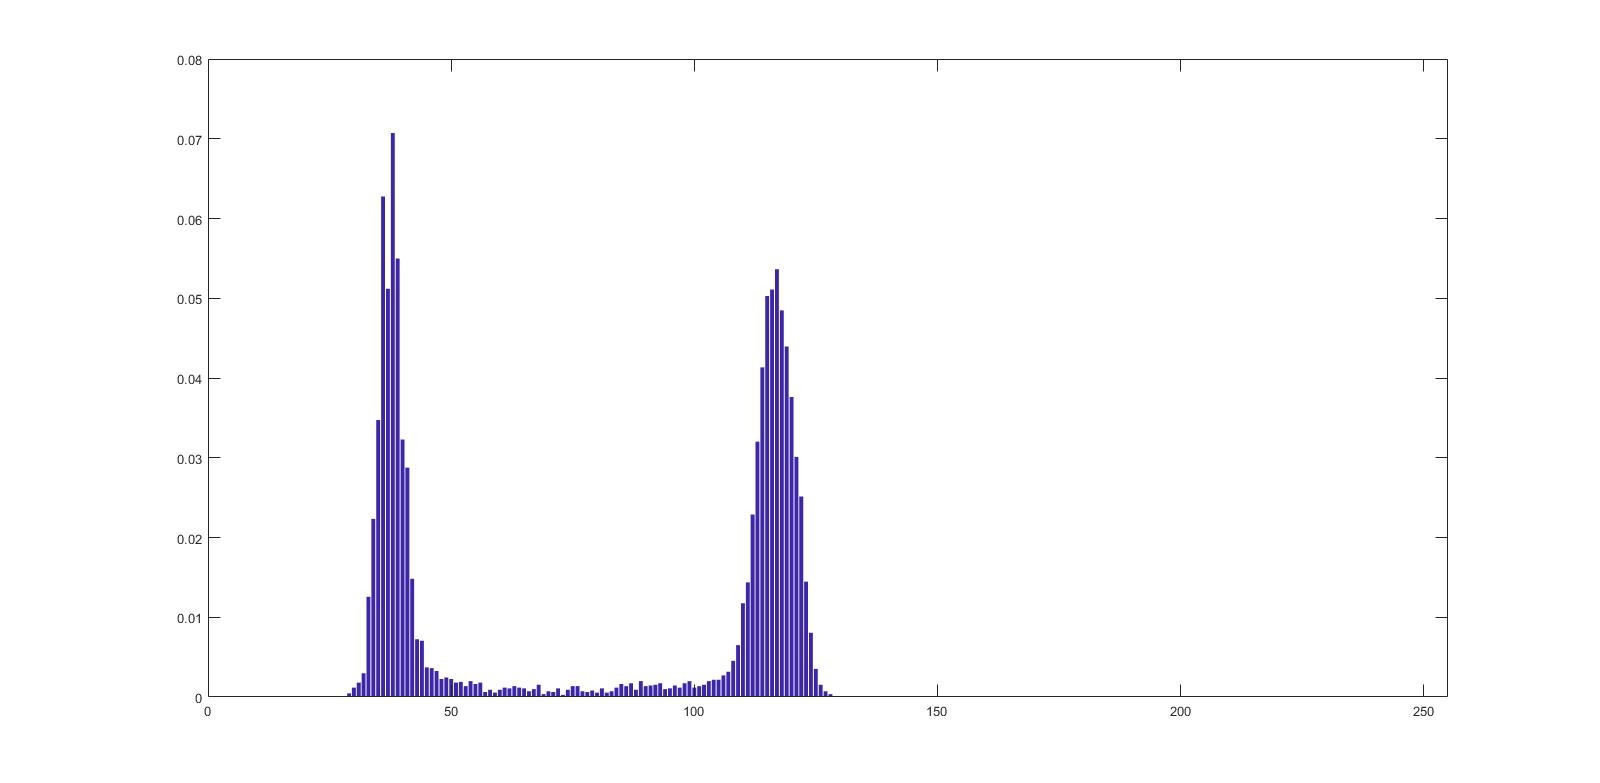
\includegraphics[width=0.98\textwidth]{bw_hist1.jpg}
 		\caption{}
 		\label{fig:bw_hist1}
 	\end{subfigure}\\
 	\begin{subfigure}{0.4\textwidth}
 		\centering
 		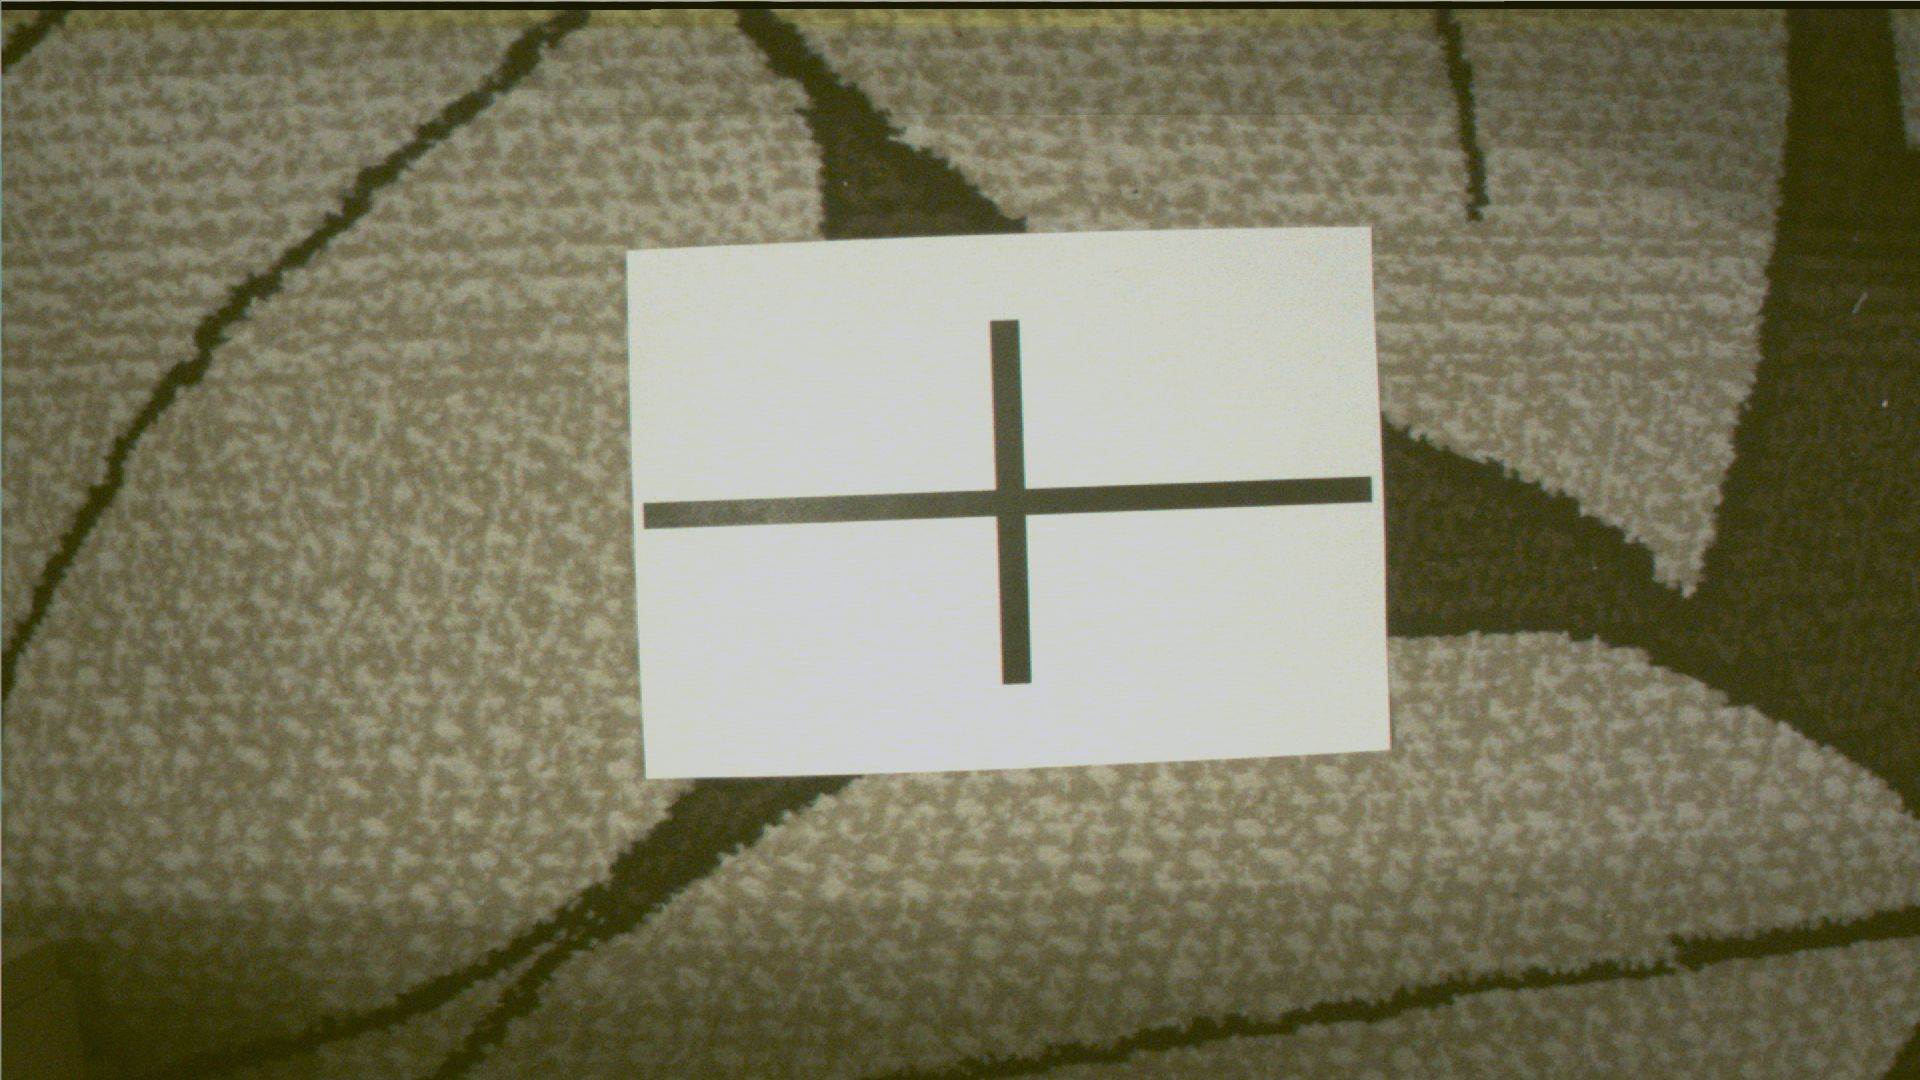
\includegraphics[width=0.98\textwidth]{rgb_sredni.jpg}
 		\caption{}
 		\label{fig:osw2}
 	\end{subfigure}
 	\begin{subfigure}{0.55\textwidth}
 		\centering
 		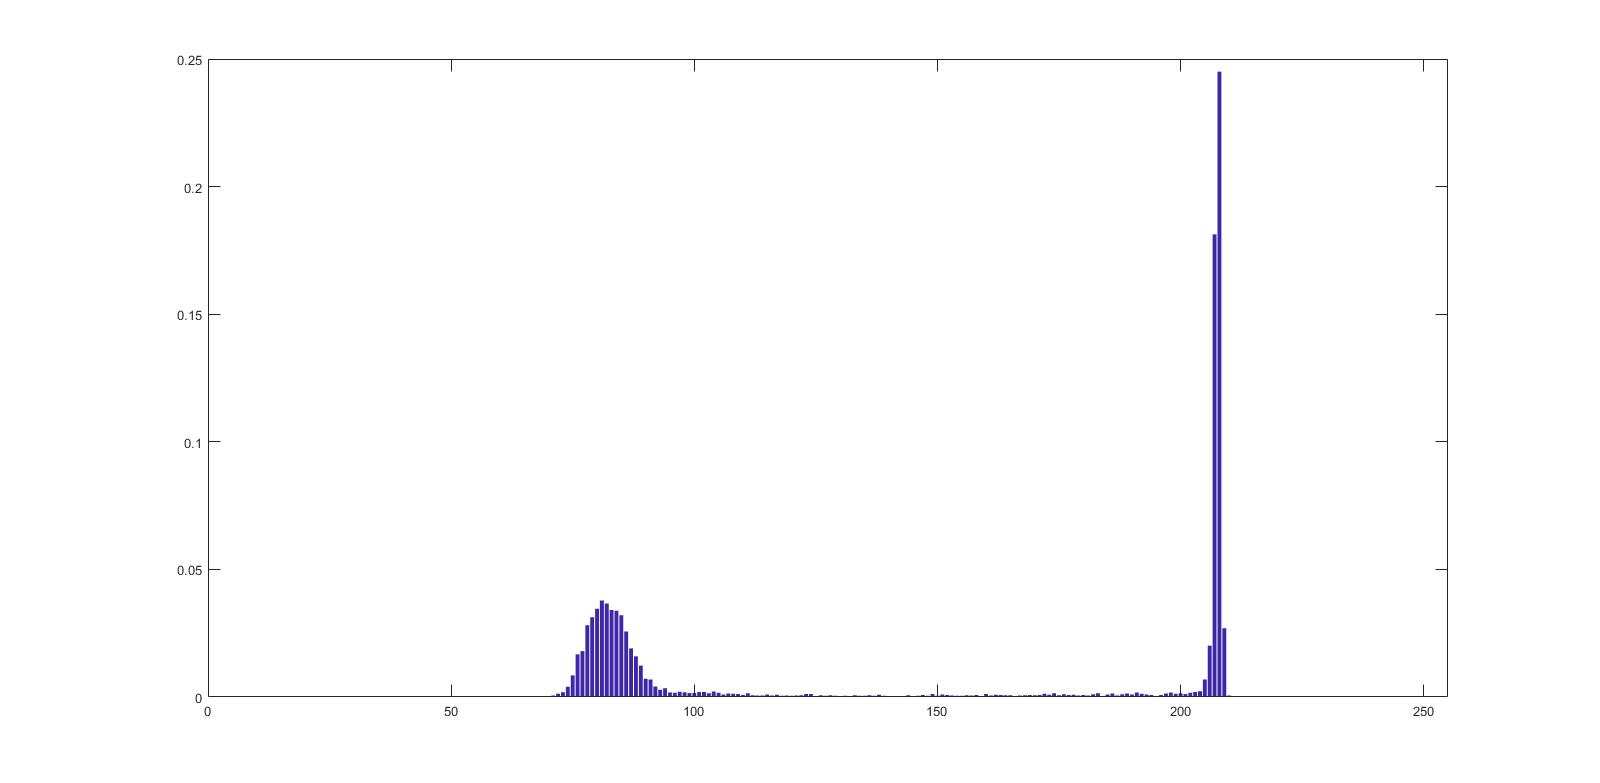
\includegraphics[width=0.98\textwidth]{bw_hist2.jpg}
 		\caption{}
 		\label{fig:bw_hist2}
 	\end{subfigure}\\
 	\begin{subfigure}{0.4\textwidth}
 		\centering
 		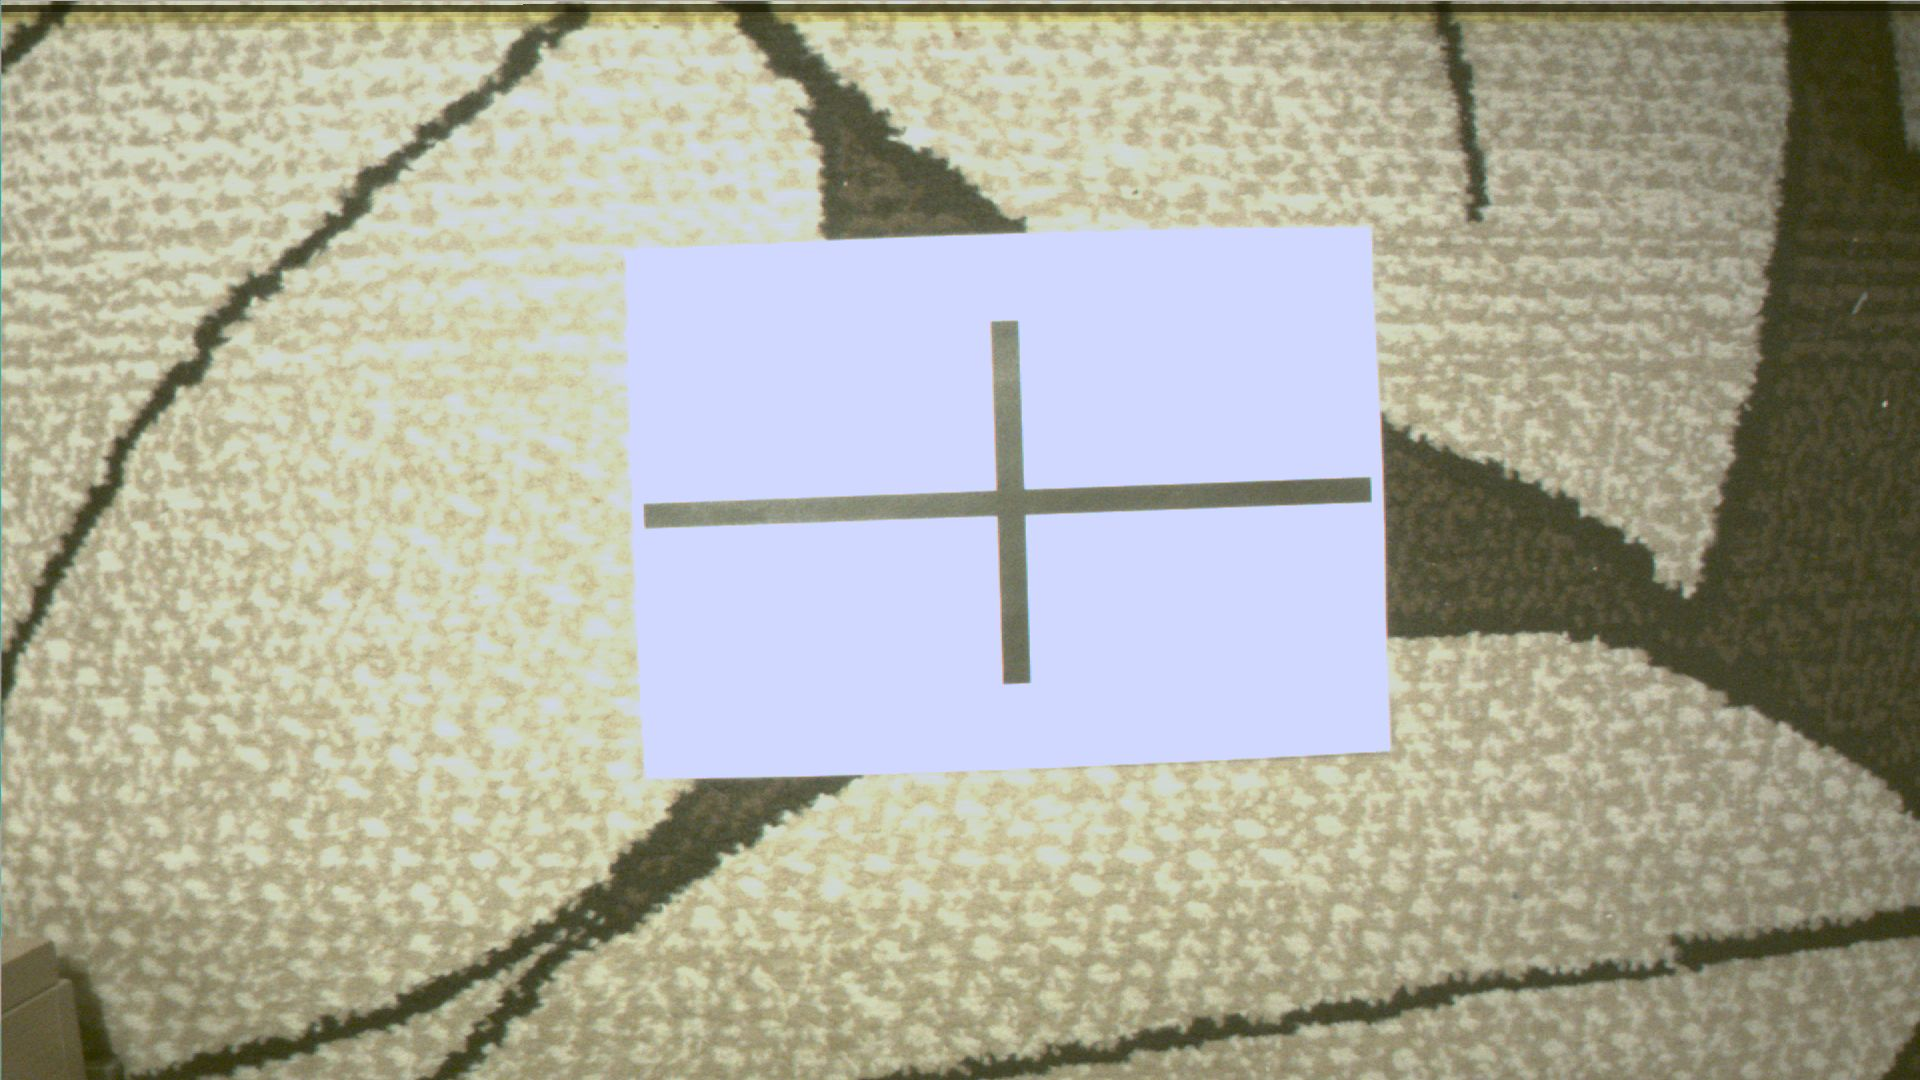
\includegraphics[width=0.98\textwidth]{rgb_jasny.jpg}
 		\caption{}
 		\label{fig:osw3}
 	\end{subfigure}
 	\begin{subfigure}{0.55\textwidth}
 		\centering
 		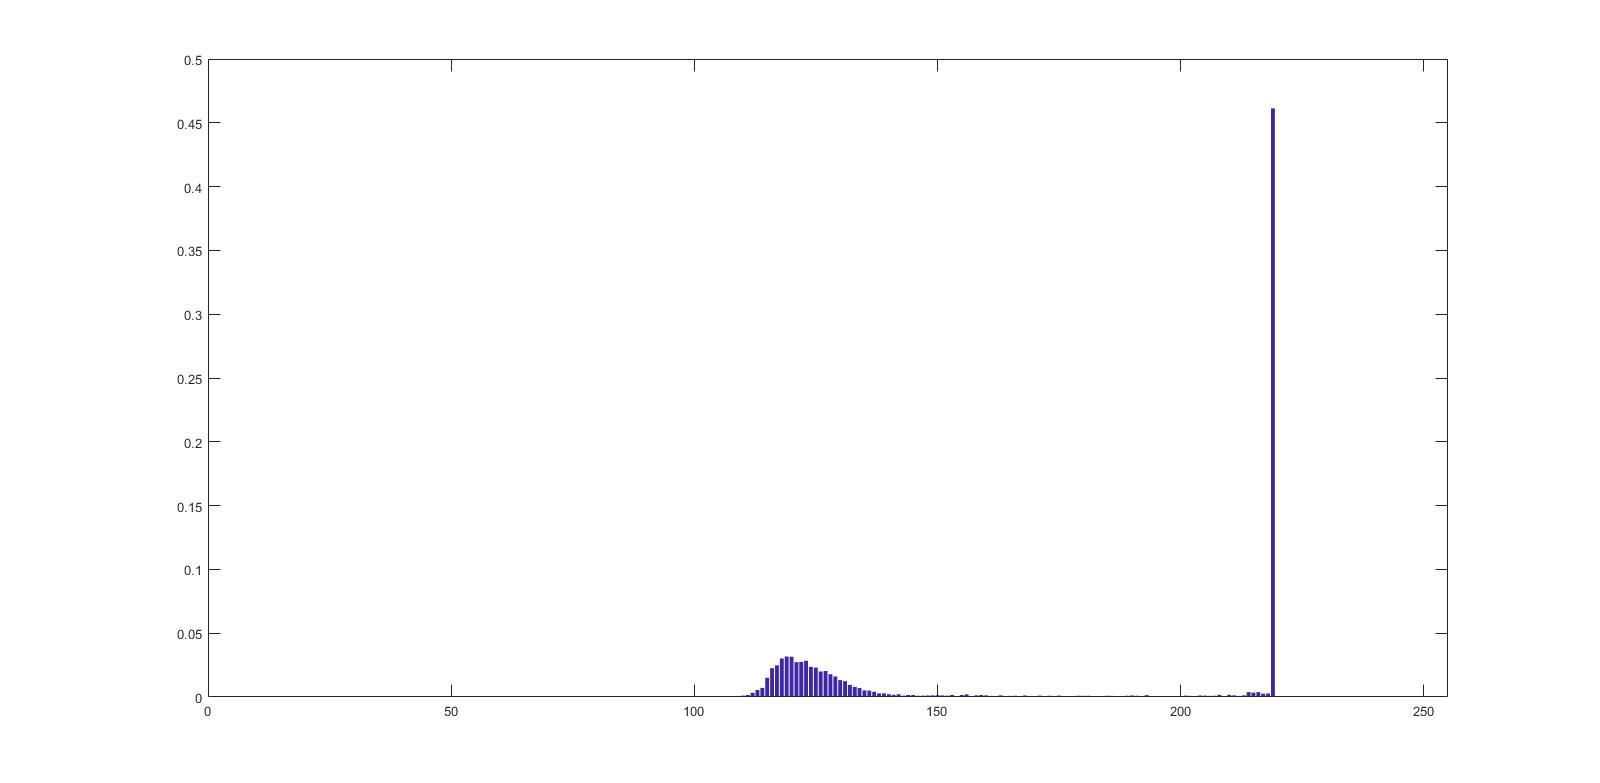
\includegraphics[width=0.98\textwidth]{bw_hist3.jpg}
 		\caption{}
 		\label{fig:bw_hist3}
 	\end{subfigure}
 	\caption{Zdjęcia pierwszej wersji znacznika wraz z~histogramami obszaru znacznika}
 	\label{fig:zdjecia_wejsciowe}
 \end{figure}

 Analiza histogramów wskazuje na~silne uzależnienie wartości koloru od~oświetlenia. Dla kolejnych obrazów, wartości progów binaryzacji mogłyby zawierać się w~zakresach: 50-100, 100-200, 150-210. Poziom białego tła dla obrazka najsłabiej oświetlonego jest mniejszy niż wartość czarnego koloru znacznika najlepiej oświetlonego. W~takiej sytuacji niemożliwy jest dobór stałego progu umożliwiającego skuteczną binaryzację.\par
 Z~tego powodu zdecydowano się na~powtórzenie eksperymentu w~przestrzeni YCbCr. Tak jak opisano w~sekcji \ref{sec:implementacja_modelu_programowego}, piksel w~tej przestrzeni opisuje współrzędna luminancji i~dwie składowe chrominacji. Podobnie jak w~przypadku RGB, przestrzeń YCbCr również da~się przedstawić w~postaci sześcianu. Tym razem skala szarości przebiega przez środek płaszczyzn Cb-Cr i~za zmianę poziomu szarości odpowiada współrzędna luminancji (Rys. \ref{fig:szescian_ycbcr}). Dla~każdej wartości piksela informacja o~jasności oddzielona jest od~barwy.\\
 Kolor znacznika określono jako czerwony, natomiast tło niebieskie, gdyż te~barwy znajdują się na~przeciwnych stronach płaszczyzny Cr-Cb. Zdjęcia wykonano przy takich samych poziomach oświetlenia jak poprzednio. Histogramy kolejnych obrazów przedstawiono na~Rys. \ref{fig:ycbcr_hist1}, \ref{fig:ycbcr_hist2}, \ref{fig:ycbcr_hist3}. 
\begin{figure}
	\centering
	\begin{subfigure}{\textwidth}
		\centering
		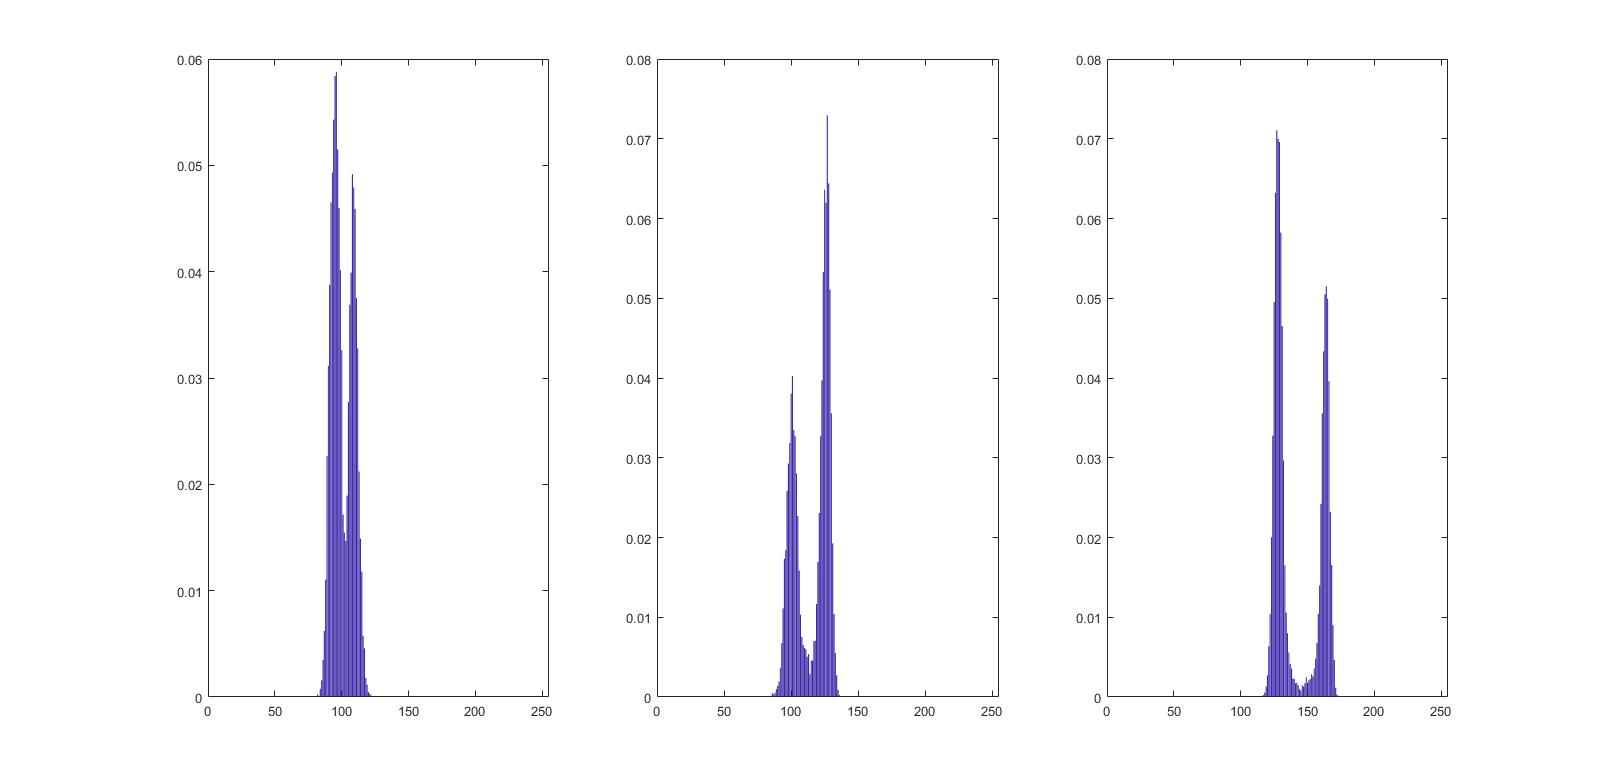
\includegraphics[width=0.9\textwidth]{ycbcr_hist1.jpg}
		\caption{}
		\label{fig:ycbcr_hist1}
	\end{subfigure}\\
	\begin{subfigure}{\textwidth}
		\centering
		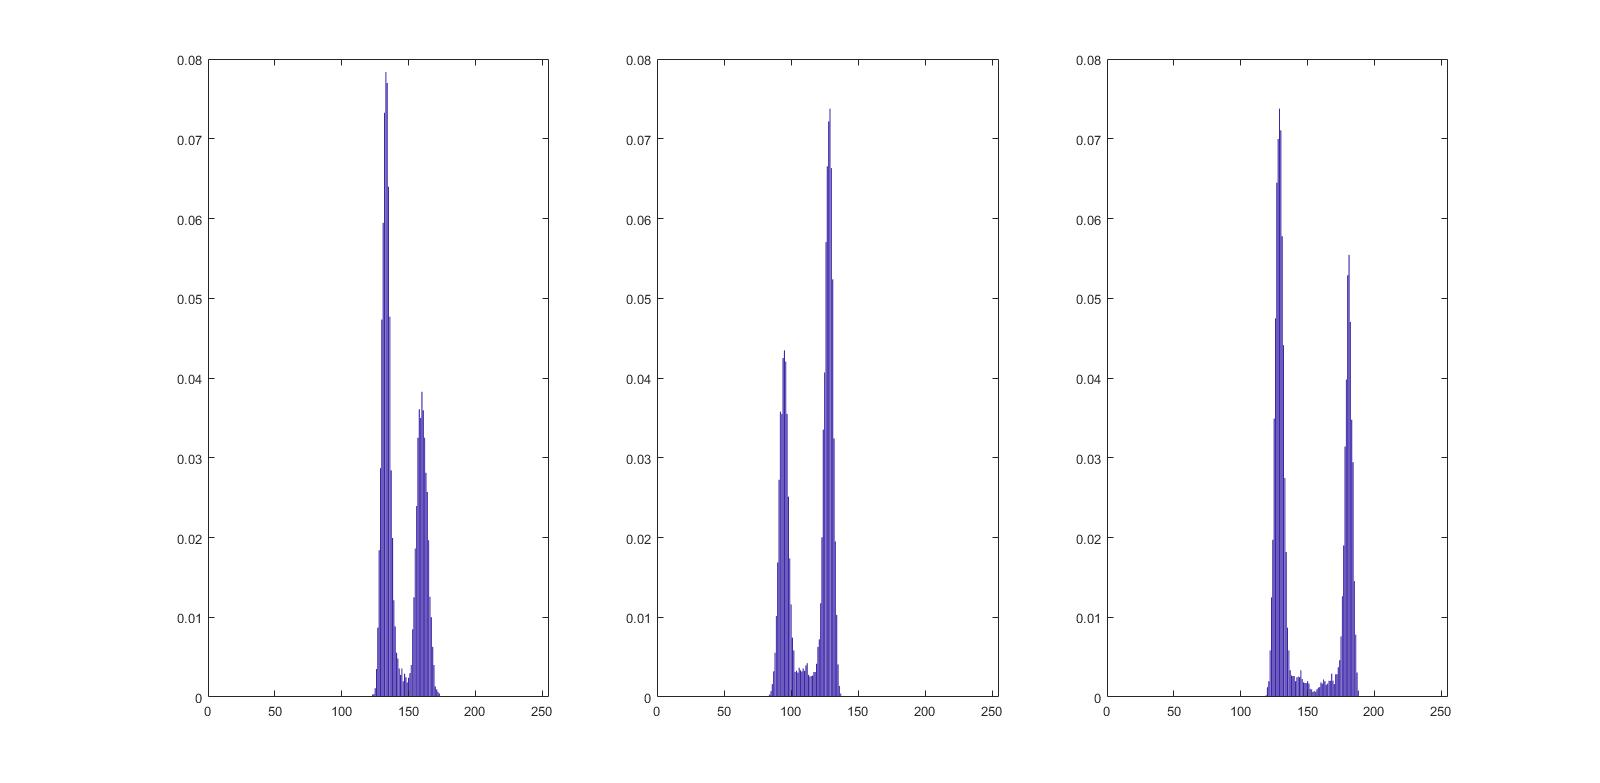
\includegraphics[width=0.9\textwidth]{ycbcr_hist2.jpg}
		\caption{}
		\label{fig:ycbcr_hist2}
	\end{subfigure}\\
	\begin{subfigure}{\textwidth}
		\centering
		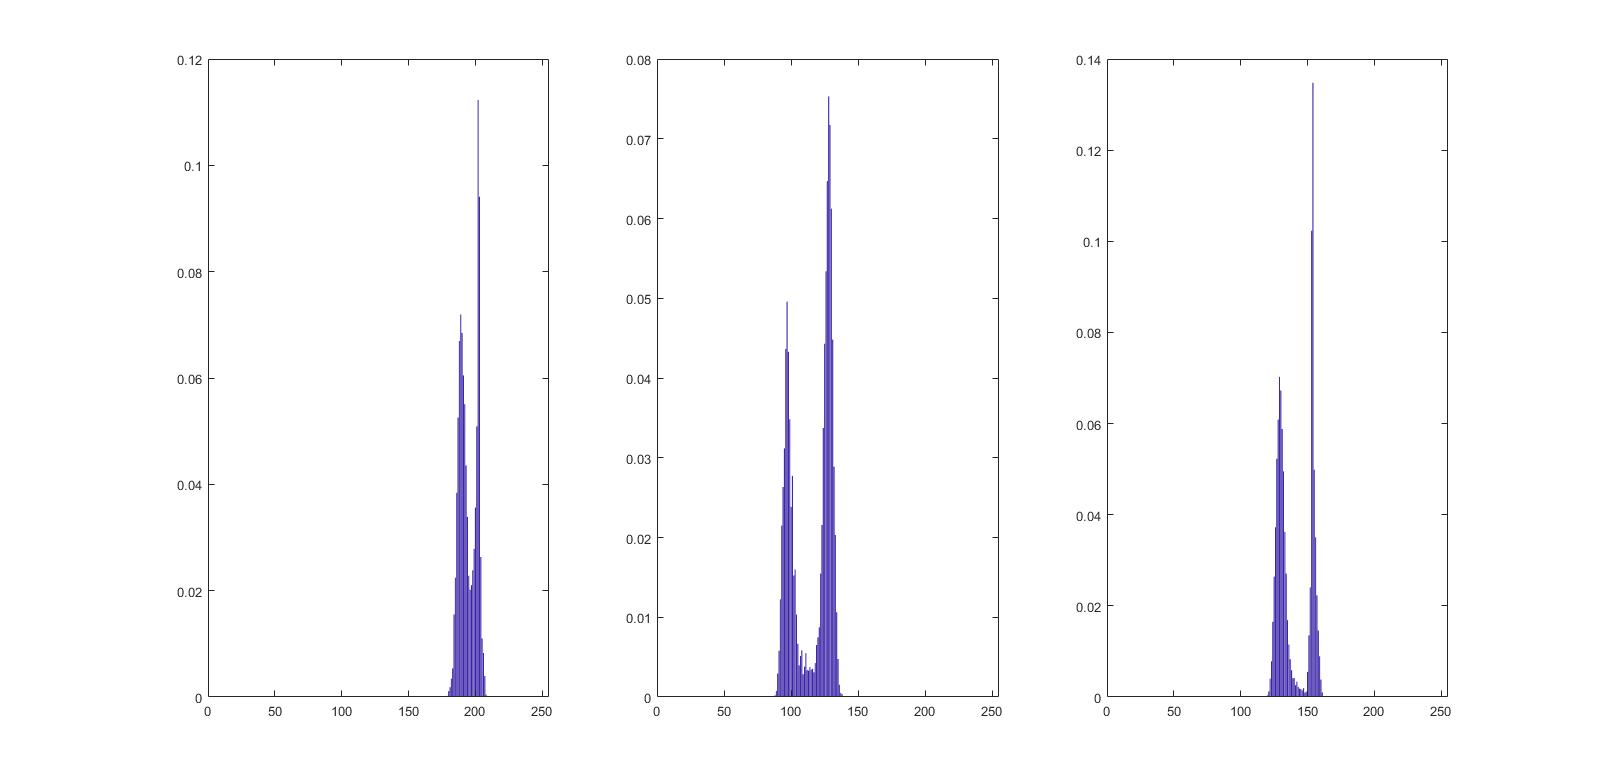
\includegraphics[width=0.9\textwidth]{ycbcr_hist3.jpg}
		\caption{}
		\label{fig:ycbcr_hist3}
	\end{subfigure}
	\caption{Histogramy obszarów znacznika w~przestrzeni YCbCr.}
	\label{fig:histogramy_ycbcr}
\end{figure}
Zgodnie z~oczekiwaniami, zmiana poziomu oświetlenia przełożyła~się na~zmianę wartości luminancji, natomiast składowe chrominancji nie zmieniały się znacząco. Każdy z~obrazów może być skutecznie zbinaryzowany przy użyciu stałych progów: górnego 120 dla składowej Cb i~dolnego 150 dla składowej Cr. Różnice pomiędzy wartościami składowych dla znacznika i~tła nie są jednak duże -- wynoszą około 30. Z~tego powodu postarano się o~możliwość szybkiego dostrojenia progów bez konieczności ponownej generacji pliku konfiguracyjnego układu (sekcja \ref{subsec:Binaryzacja}). Ostatecznie zdecydowano się na~znacznik przedstawiony na~Rys. \ref{fig:znacznik}.
\begin{figure}[h]
	\centering
	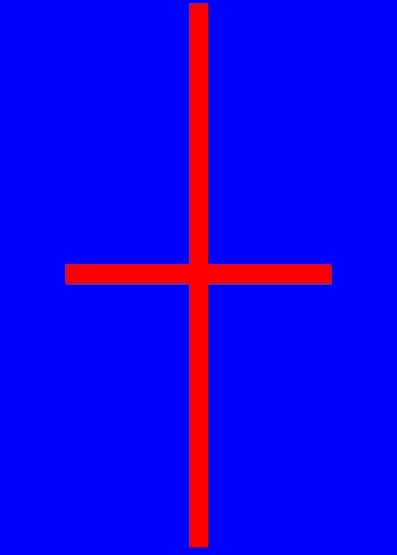
\includegraphics[width=0.3\textwidth]{znacznik.jpg}
	\caption{Wybrany wygląd znacznika}
	\label{fig:znacznik}
\end{figure}

\iffalse
\section{Wyznaczenie kąta widzenia kamery przy różnych ustawieniach rozdzielczości}
\label{sec:wyznaczenie_kata_widzenia_kamery_przy_roznych_ustawieniach}
W~celu zbadania kąta widzenia kamery stworzono moduł nakładający na~obraz prostopadłe linie przechodzące przez jego środek. %TODO dla mnie to brzemi niejasno
Następnie umieszczono kamerę na wysokości 49 cm i~skierowano ją w~dół. 
Odczytanie odległości od~środka obrazu do~jego krawędzi w~poziomie i~pionie pozwoliło na wyznaczenie kątów widzenia kamery. 
Skorzystano ze wzoru \eqref{eq:kat}.
\begin{equation}
\label{eq:kat}
\alpha=\arctan{\frac{l}{h}}
\end{equation}
gdzie:
\begin{eqwhere}[2cm]
	\item[$\alpha$] kąt widzenia kamery,
	\item[$h$] wysokość, na jakiej umieszczona jest kamera,
	\item[$l$] odległość środka obrazu od jego krawędzi.
\end{eqwhere}
Na podstawie obrazu przedstawionego na rysunku \ref{fig:1080p} obliczono kąty widzenia kamery w~pionie i~poziomie dla rozdzielczości 1920 x 1080. 
Dla rozdzielczości 1280 x 720 skorzystano z~obrazu pokazanego na rysunku \ref{fig:720p}. 
Korzystając ze wzoru \eqref{eq:kat} otrzymano przybliżone wyniki, przedstawione w tabeli \ref{tab:rozdzielczosc}.
\begin{table}[]
	\caption{Wartości kąta widzenia kamery w zależności od rozdzielczości}
	\label{tab:rozdzielczosc}
	\centering
	\begin{tabular}{|c|c|c|}
		\hline
		\begin{tabular}[c]{@{}c@{}}Rozdzielczość\end{tabular} &  Kąt widzenia kamery w pionie w stopniach  &  Kąt widzenia kamery w poziomie w stopniach  \\ \hline
		1920 x 1080                                                                          & 14 & 27 \\ \hline
		1280 x 720                                                                         & 19 & 38 \\ \hline
	\end{tabular}
\end{table}
\begin{figure}[h]
	\centering
	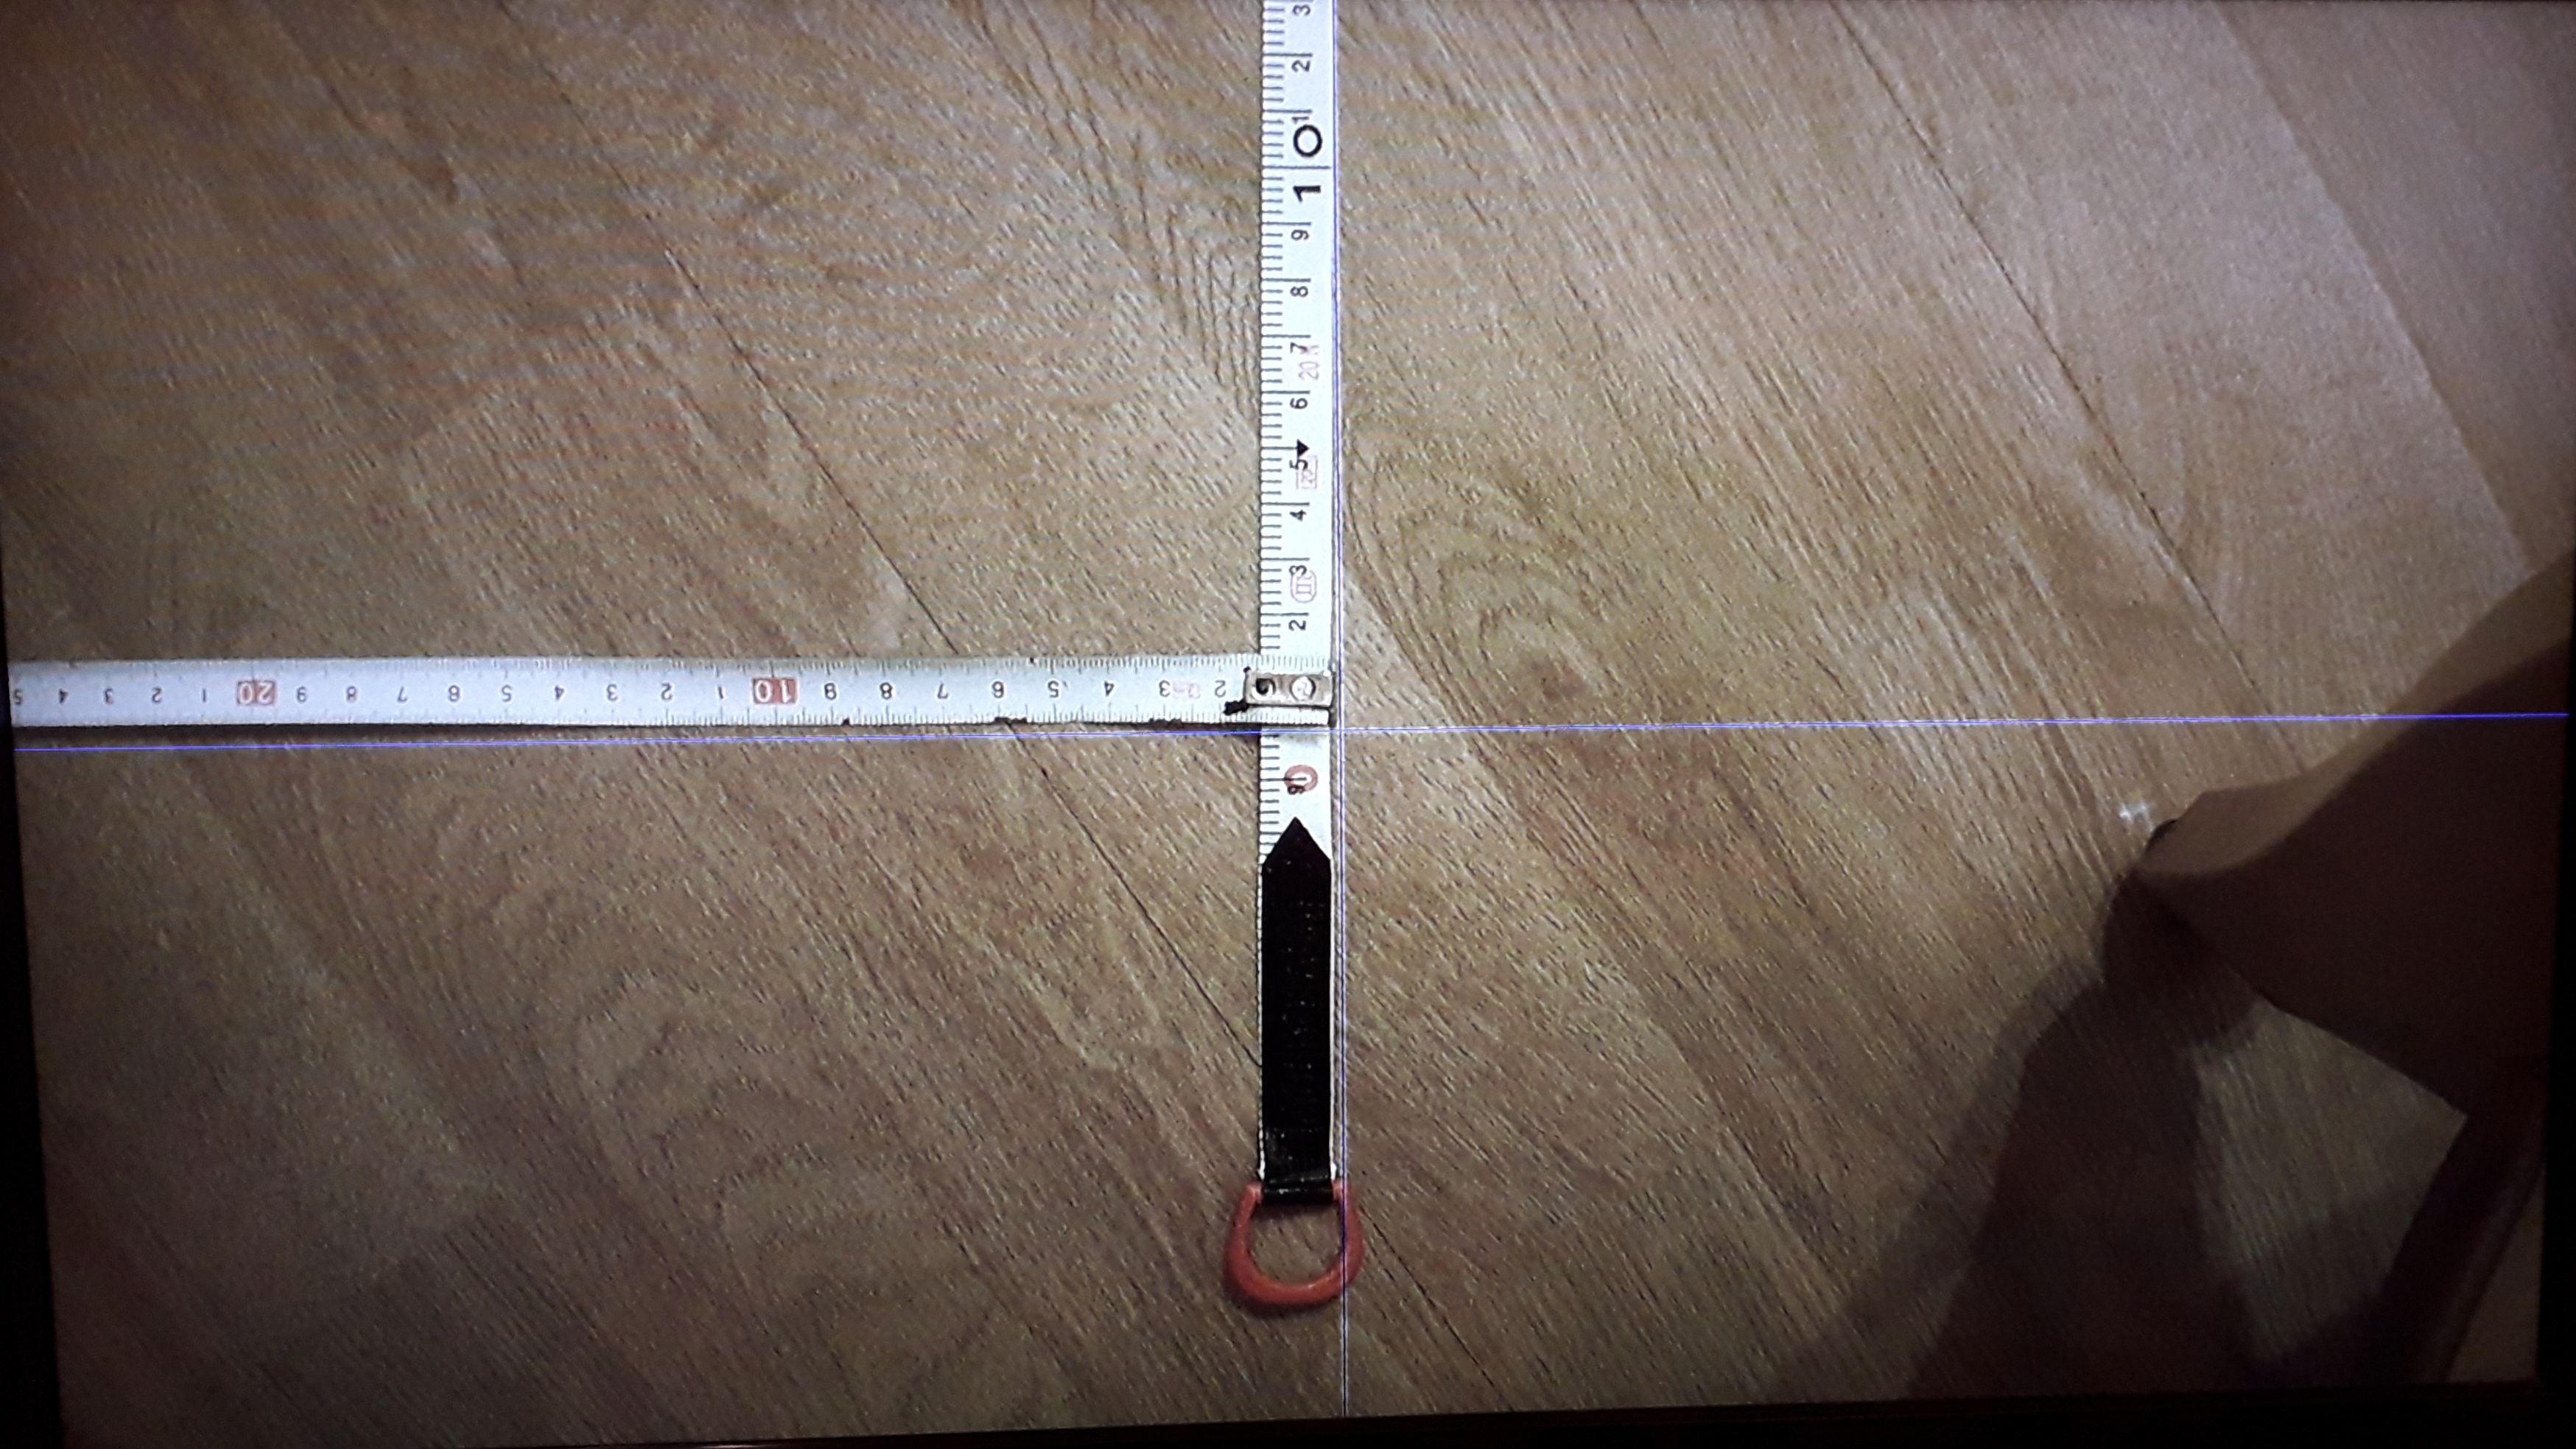
\includegraphics[width=\textwidth]{1080p.jpg}
	\caption{Obraz służący do wyznaczenia kąta widzenia kamery dla rozdzielczości 1920 x 1080.}
	\label{fig:1080p}
\end{figure}
\begin{figure}[h]
	\centering
	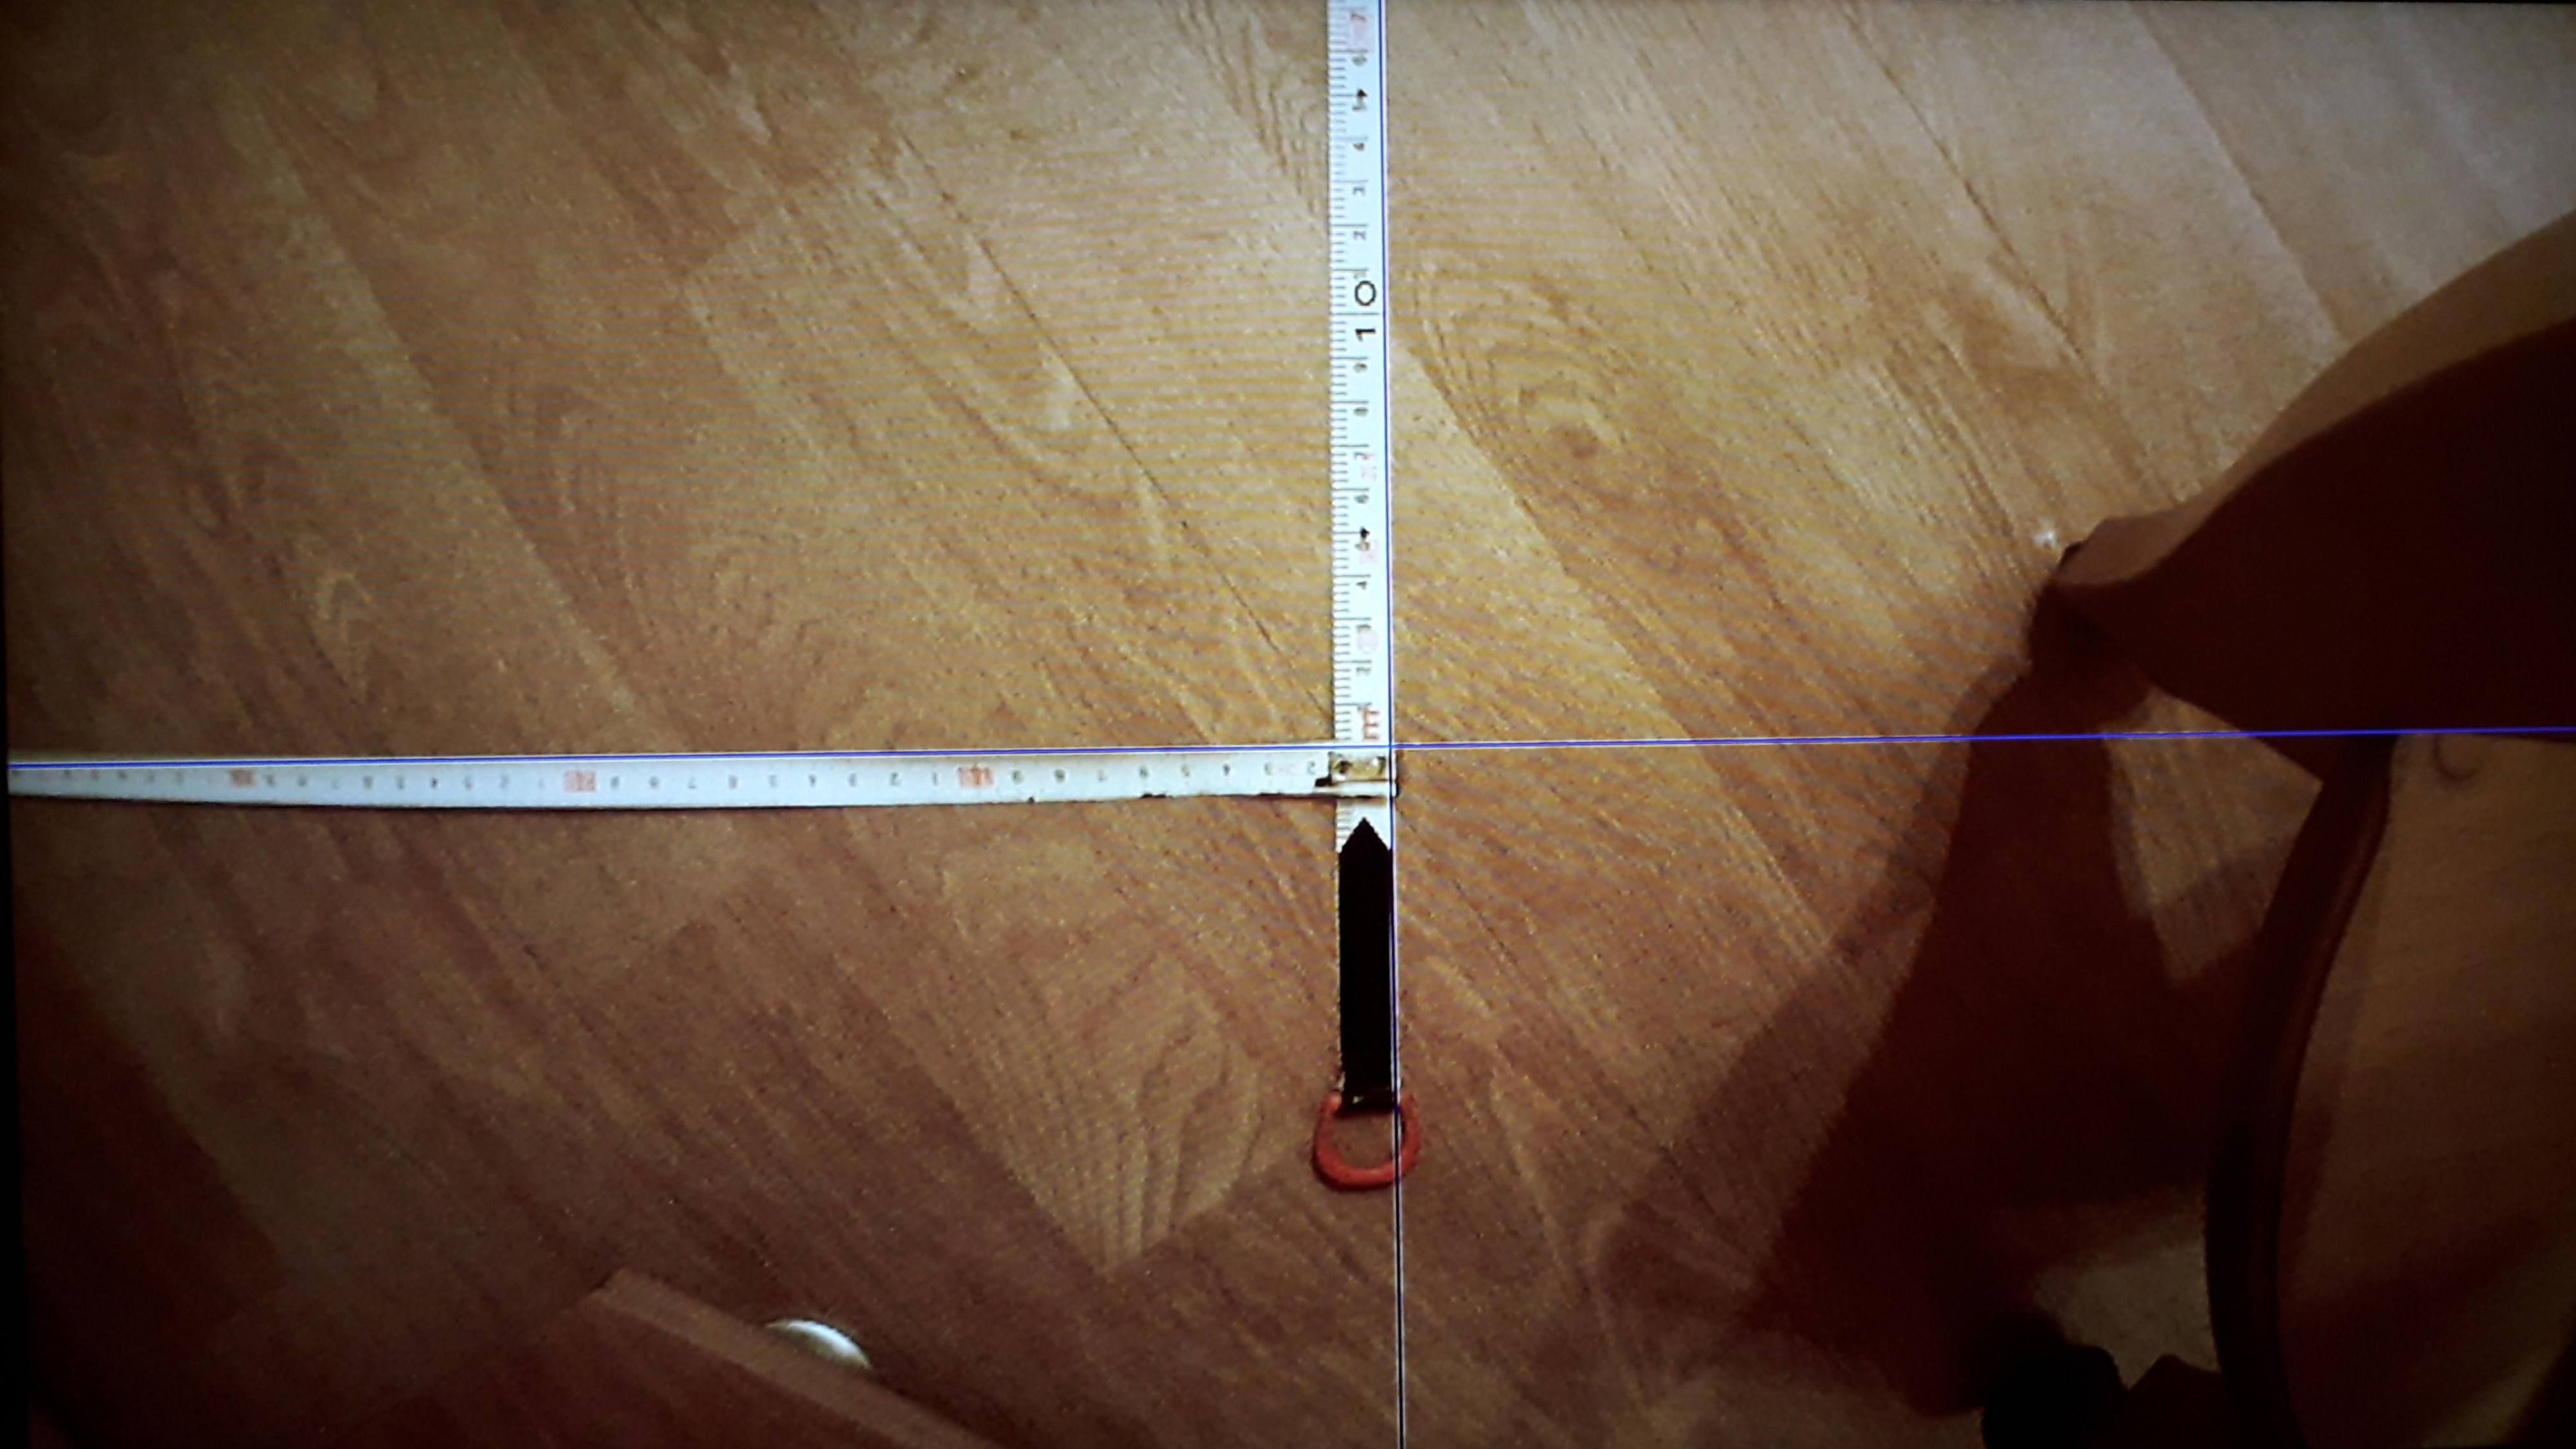
\includegraphics[width=\textwidth]{720p.jpg}
	\caption{Obraz służący do wyznaczenia kąta widzenia kamery dla rozdzielczości 1280 x 720.}
	\label{fig:720p}
\end{figure}

%TODO Jakieś wnioski...
\fi

\section{Test regulacji położenia drona}
\label{sec:test_regulacji_polozenia_drona}
--- Test będzie polegał na zadawaniu prędkości w x i y proporcjonalnej do liczby pikseli dzielącej środek obrazu od aktualnego położenia znacznika. 
Celem będzie doprowadzenie do sytuacji stabilnego unoszenia drona nad znacznikiem. 
Rejestrowanie uchybu w x i y i ich zapis na kartę SD pozwoli na sporządzenie wykresów tych wartości w czasie.

\section{Lądowanie na nieruchomym lądowisku}
\label{sec:ladowanie_na_nieruchomym_ladowisku}
--- Do poprzedniego testu zostanie dodana funkcjonalność lądowania.
%---------------------------------------------------------------------------
%---------------------------------------------------------------------------
